\section{Introduction}

\begin{figure*}[t] 
    \centering 
    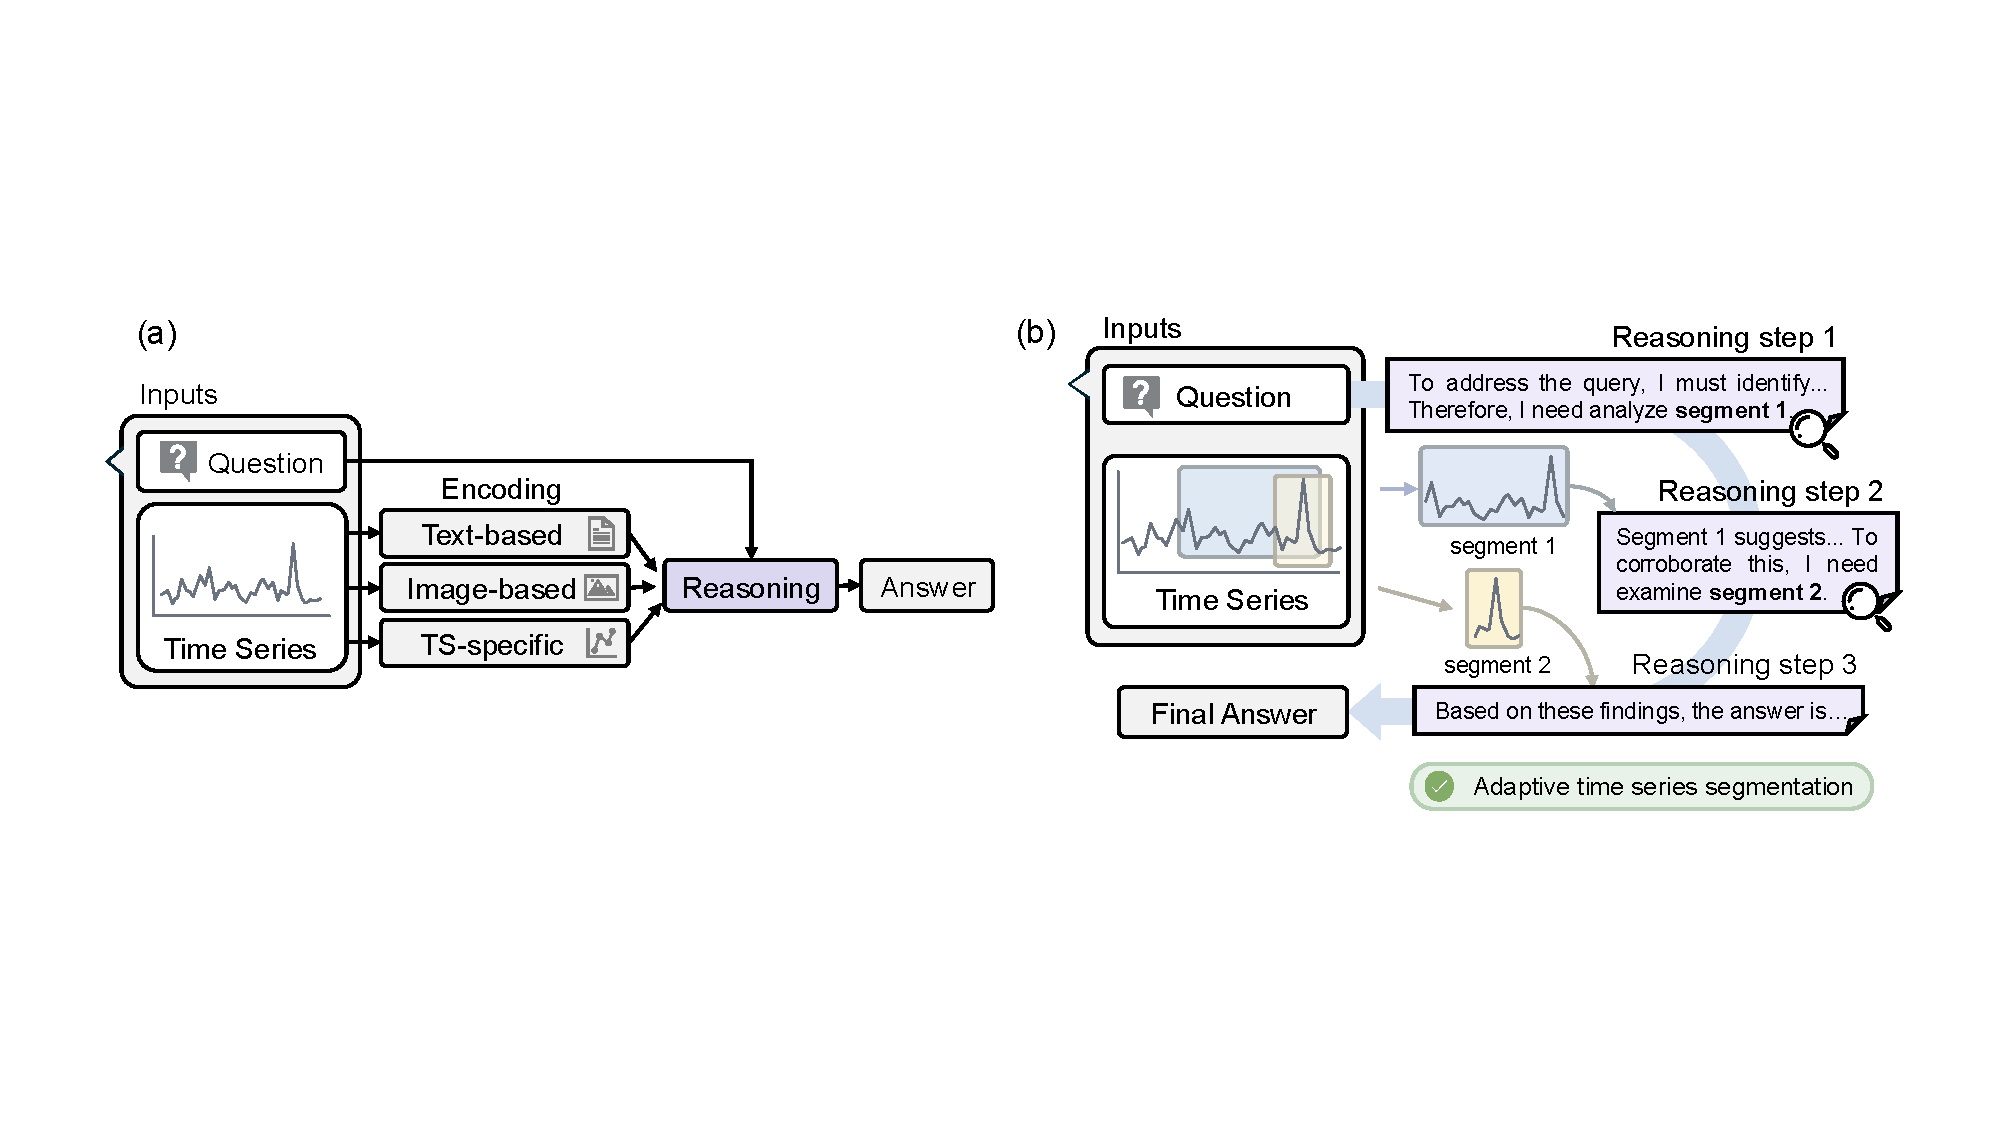
\includegraphics[width=0.9\textwidth]{figs/fig1_motivation.pdf} 
    \caption{
    %
     (a) Time-series reasoning: answering a natural language question given a time series. (b) \algoname alternates between reasoning and adaptive segment selection, choosing the next segment based on the question and intermediate outputs, and stopping once it can produce the final answer.
    }
    \vspace{-5mm}
    \label{fig:main} 
\end{figure*}

Time-series modeling has long been shaped by tasks such as forecasting~\cite{das2024decoder,he2025sempo,yang2025not,wang2025toward}, classification~\cite{liu2025learning_cls,liu2025sarc,tran2025mix}, and anomaly detection~\cite{sun2025sunmultivariate,cai2025caiself,kim2025causality}. Increasingly, however, real-world use cases begin with a natural-language question rather than a predefined label or prediction horizon. A clinician may ask why a patient’s vital signs deteriorated after a medication change, and an analyst may ask what triggered a regime shift in a market indicator. Answering these questions requires linking the question to patterns in the time series and grounding the answer in relevant segments. This emerging setting, known as time series reasoning~\cite{chow2024towards,kong2025position}, asks models to answer natural language questions by identifying and analyzing the task-relevant parts of a time series.

Recent work has examined how to interface time series with large language models (LLMs). As in Figure~\ref{fig:main}a, approaches mainly differ in how they convert a time series into an LLM input, including textual serialization~\cite{alnegheimish2024large,luo2025time,liu2025can}, rendered plots~\cite{rcw_dataset,zhang2025timemaster}, and learned embeddings~\cite{chatts,itformer,langer2025opentslm}. These designs improve modality alignment but keep inference static: the model receives a fixed view of the full time series and must answer from that view. This is limiting for multi-step reasoning, where intermediate conclusions should change what the model inspects next. For example, a clinical deterioration query may first check for an abrupt spike, then shift to a different window or a narrower interval to test a hypothesis. More broadly, relevant temporal segments are query- and step-dependent. Figure~\ref{fig:main}b shows the desired behavior: reasoning interleaved with temporal segment selection, stopping when the model is ready to answer.

A key missing capability is question-adaptive information selection during inference. Time series inputs are long and temporally heterogeneous, and the same sequence can support many different questions that require different regions and different resolutions. As a result, forcing the model to process a fixed view of the full series can dilute salient local structure and, in long sequences, can degrade performance by mixing irrelevant context with task-relevant information. Related problems have been studied in text-vision reasoning, where models learn to search or zoom into regions conditioned on intermediate steps~\cite{wang2025pixel,zhang2025chain,li2025imagine}. However, an analogous mechanism for time-series reasoning remains underexplored, despite the strong need for adaptive localization in long  time series.

Two challenges make question-adaptive segment selection difficult in time series reasoning. First, unlike images, time series rarely include task-agnostic annotations that identify segments relevant to a given question. Relevant segments depend on the question, so the model must decide during inference which parts of time series to inspect.
Second, many post-training methods use reinforcement learning to optimize sequential decision making at the level of output tokens (e.g., PPO~\cite{schulman2017ppo}, GRPO~\cite{shao2024deepseekmath}, DAPO~\cite{yu2025dapo}). Token-level optimization becomes difficult when a task requires multiple sub-tasks and the reasoning horizon is long. Credit assignment then becomes diffuse: key steps such as tool calls or information selection occupy only a small part of the token sequence, so their effect on final output is hard to isolate and optimize. Approaches that disentangle traces into components and optimize them with role-specific objectives can target these steps directly~\cite{klissarov2025hrl}. This motivates our present work on separating temporal segment acquisition from time series answer generation.

\xhdr{Present work}
%
\algoname\footnote{ARTIST website: \url{https://zitniklab.hms.harvard.edu/ARTIST/}; code: \url{https://github.com/mims-harvard/ARTIST}} (Adaptive Reasoning for TIme-Series via Temporal Selection) is a time-series reasoning approach where an LLM is trained to treat time series as an active resource during inference (Figure~\ref{fig:main}). It interleaves reasoning with temporal segment selection by training a single policy to operate in two roles. A high-level \emph{controller} selects the next segment and decides when to stop, conditioned on the question and intermediate outputs. A low-level \emph{reasoner} produces intermediate reasoning steps and the final answer conditioned on the selected segments. This separation explicitly decouples \emph{where to look} from \emph{how to reason}.
%
\algoname is trained in two stages. First, we apply supervised fine-tuning (SFT) on curated traces that interleave segment selection with natural language reasoning. Second, we use collaborative self-play reinforcement learning to jointly optimize both roles. The controller is trained with a reliability-based reward that measures answer consistency under repeated sampling, and the reasoner is trained for correctness and format compliance conditioned on controller-selected segments.
Across six benchmarks in clinical, financial, environmental, and general domain time series reasoning, \algoname outperforms large language models, vision-language models, and prior time-series reasoning systems. It achieves an average accuracy improvement of 6.46 percentage points over the strongest comparator, with gains of up to 12.5 points on datasets requiring localized or multi-segment reasoning. Supervised fine-tuning alone yields an average accuracy increase of 5.65 points over  baselines, while reinforcement learning provides additional gains by optimizing question-adaptive segment selection. Further, \algoname typically uses only 30-70\% of the input time series sample per query, showing that selective temporal analysis improves accuracy without requiring full time series consumption.

\xhdr{Contributions}
(1) We present adaptive segment selection for time series reasoning. The model iteratively chooses temporal segments to inspect and updates its reasoning based on the retrieved segments. This setting does not assume pre-defined segment labels.
(2) We introduce a hierarchical, collaborative self-play RL post-training method that separates segment selection from answer generation and trains each role with learning signals aligned to its role.
(3) On six benchmarks, \algoname outperforms seven strong baselines. It improves average accuracy by 6.46 absolute percentage points over the strongest comparator while using a smaller fraction of the input time series.

\xhdr{Conflict of Interest Disclosure}
The authors declare no financial conflicts of interest or other substantive conflicts that could reasonably be perceived to influence the work presented in this paper.